\documentclass{wsuthesis-1e} % use the "twoside" option for two-sided printing
\usepackage{amsmath,amsfonts} % math stuff
\usepackage{graphicx} % figures stuff
\usepackage{rotating} % sideways figure stuff

%% uncomment or comment to print the nomenclature page
\nomenclaturepagetrue

\begin{document}
\title{How to Write Theses\\
  With Two Line Titles}
\author{John Henry Candidate}
\thesistype{thesis}
\engineeringtype{Electrical}
\principaladvisor{Jill Parker}
\firstreader{John Green}
\secondreader{Jane Doe}
% \thirdreader{Jane Supernumerary} %if needed
% \fourthreader{Severus Snape} %if needed

\beforepreface
\prefacesection{Dedication}

The Dedication page is optional and follows the Title Page. Preliminary pages which precede the Table of Contents, include the Dedication, are not displayed in the Table of Contents.   The text in the Dedication is limited to one page and is in the same font size and style as the other text in the project report/thesis.



%%% Local Variables:
%%% mode: latex
%%% TeX-master: "../thesis_template_test"
%%% End:



\afterpreface
\nomenclature{$c$}{Speed of light in a vacuum inertial frame}
\nomenclature{$h$}{Planck constant}
\nomenclature{SS-FSE}{Single-Shot Fast Spin Echo}



%%% Local Variables:
%%% mode: latex
%%% TeX-master: "../thesis_template_test"
%%% End:

\prefacesection{Acknowledgements}

The Acknowledgements page is optional and limited to four pages. It precedes the Abstract page. Heading is bold if other major headings are bold. It is in the same font size and style as text, and the vertical spacing, and paragraph style margins are the same as used in text. Use complete sentences.

An example would be something along the lines of:   I would like to thank my committee chair, Professor Smith, and my committee Professor Johns and Professor Williams, for their guidance and support throughout the course of this research.
In addition, I would also like to thank my friends, colleagues, and the department faculty and staff for making my time at Weber State University a positive experience...



%%% Local Variables:
%%% mode: latex
%%% TeX-master: "../thesis_template_test"
%%% End:

\prefacesection{Abstract}

The text of the Abstract is double-spaced or space-and-a-half according to the spacing style of the text of the project report/thesis. Follow the same margin settings as your narrative text. The page number (lower case Roman numeral) should be placed at the top center of the page.

Your Abstract must be a ``complete snapshot'' of your manuscript and be a stand-alone piece. Since the text of the Abstract may be distributed widely through a variety of databases, formal citations, images, and complex equations should not be included. Paragraph one introduces your specific problem and the methods used. The remaining paragraphs present the research and results in detail.

%%% Local Variables:
%%% mode: latex
%%% TeX-master: "../thesis_template_test"
%%% End:

\startchapters
\chapter{Introduction: Formatting}
\label{cha:introduction}

New chapters always start on a new page.  Number chapters using Arabic numbers. Avoid excessive white space on your pages. There should be no more than one-quarter to one-third of a page that is blank.

Paragraphs of the body text are all indented.  Text is double spaced. Being consistent is very important in formatting your project report/thesis. Use the same formatting basics in all the chapters. Always leave at least two lines of text at the bottom of a page or at the top of a page. If it is less than two lines, then force a page break earlier.

\section{Typeface and Spacing}
\label{sec:typeface-spacing}

Text should be 11-point or 12-point in a serif font. Line spacing should be double. Typeface, size and spacing should be consistent throughout the document. Major sections should be titled and numbered. Subsections should be titled using subsequent subsection numbers (1.1, 1.2, etc.).

\section{Margins and Page Numbers}
\label{sec:margins-page-numbers}

All margins except for the binding edge should be 1''. The binding edge (left margin) should be 1.5''.  Each page (except the cover page and the appendices) should be numbered in the bottom margin. The page number may be centered or justified on the side opposite the binding edge. Page numbers should either be a single page number or a section number and a page number separated by a dash. Lower case Roman numerals are allowed on introductory pages.

\section{Floats}
\label{sec:floats}

In \LaTeX\, figures are tables are placed according to ``floats.''  This section will discuss both cases and appropriate usage.  

\subsection{Figures}
\label{sec:figures}

In \LaTeX, figures are floated based on what the compiler thinks is the most optimal position.  The float property by what is in the square brackets.  Please see online documentation as to where the figures will be placed.  Generally, try to place the figures on the same page it is referenced in the text.  If it is impossible to get both figure and reference on the same page, place it after first reference.  See Fig.~\ref{fig:snowbasinPhoto} for an example.  Referencing photos in the text should follow the ``Fig. X'' format, where ``X'' is the figure number.  \LaTeX\ is very good at managing figure numbers, so please use the \verb+\label+ and \verb+\ref+ commands to manage figure numbers.

\begin{figure}[h!]
  \centering
  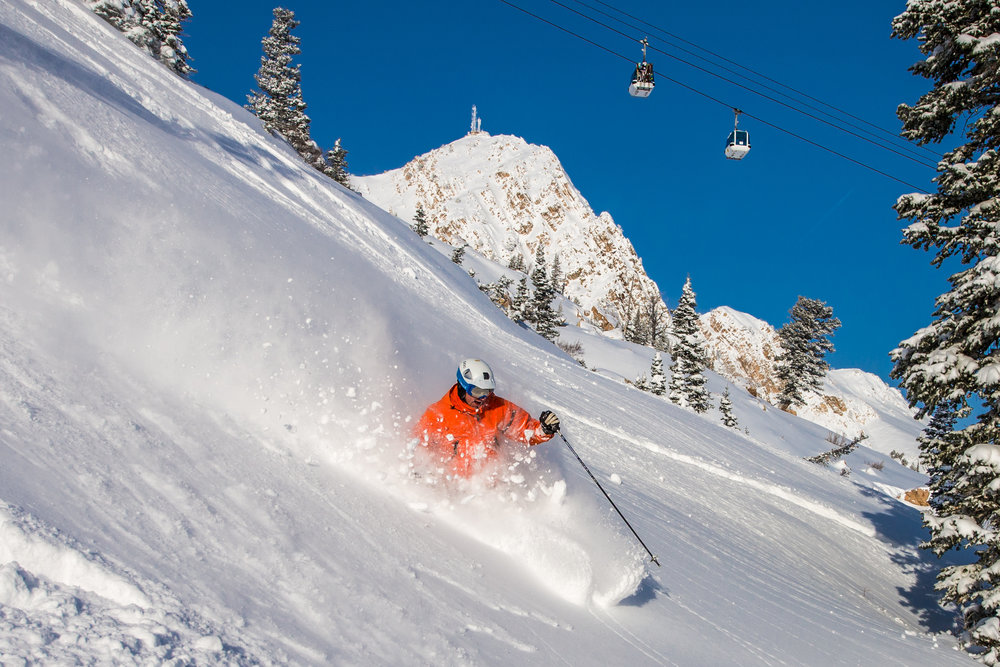
\includegraphics[width=4in]{images/snowbasin.jpg}
  \caption[Example short caption]{Example figure caption.  You can make your captions long, but for the purpose of the list of images, please include a shorter caption.}
  \label{fig:snowbasinPhoto}
\end{figure}

\subsection{Tables}
\label{sec:tables}

All tables should be numbered, either with a single table number or with a section number and a table number separated by a period. Table numbers should increment with each table in the section or document. Each table should be labeled with (a) the word Table, (b) the table number, (c) a colon and (d) a title. Table labels should be located above their respective tables.

A \LaTeX example of a table and this convention can be seen in Table~\ref{tab:exampleTable}.
\begin{table}[h!]
  \centering
  \begin{tabular}[h!]{| c | c | c | c |}
    \hline
    column 1 & column 2 & column 3 & column 4 \\
    \hline\hline
    row 1 & 1 & 2 & 3 \\
    \hline
    row 2 & 1 & 2 & 3 \\
    \hline
  \end{tabular}
  \caption[Short table caption.]{An example table.  Please see the extensive documentation online on how to make tables in \LaTeX.}
  \label{tab:exampleTable}
\end{table}

\section{Equations}
\label{sec:equations}

There are many reasons to \LaTeX\ over other word processing suites, but one of the most compelling its superior equation rendering and typesetting.  \LaTeX\ is capable of inline and block equations.  An example of inline equation is $z=x+jy$.  An example of a block equation would be
\begin{equation}
  \label{eq:1}
  F(j\omega) = \int_\mathbb{R} f(t)e^{-j\omega t}dt.
\end{equation}
One common mistake is to terminate a sentence with an equation but not include the punctuation after the equation.  If a sentence ends with an equation, it needs a period after the equation.

The decision to use an inline versus a block equation depends on a few factors.  Primarily, if the equation is long or complicated, it needs to be offset as a block equation (see Eq.~(\ref{eq:1})).  However, if the equation is short and simple, it can be left inline.  Secondarily, block equations are numbered in \LaTeX, and this numbering can be managed by the \verb+\label+ and \verb+\ref+ functions similar to the figure and table examples.  If you need to reference your equation later in the text, it should be in a numbered block equation for future referencing.

\section{References}
\label{sec:references}

All references in the bibliography should be in IEEE format. \LaTeX and BibTeX do a stellar job managing bibliographies.  Following standard practices demonstrated here will generate an appropriate bibliography.  Please refer to the source code for an example\cite{pauly1991parameter}.  There are many open-source programs to manage BibTeX files such as JabRef (Linux/Mac/Windows) and BibDesk (Mac).  Lastly, the citation goes before the period (see earlier example) as the citation is considered to be part of the sentence.

\section{Appendices}
\label{sec:appendices}

The main appendix starts on a new page at the end of the main text.  Appendix sections can also be referred to in the main text through the \verb+\label+ and \verb+\ref+ commands. See Appendix~\ref{sec:some-long-proof} as an example.

\section{Landscape}
\label{sec:landscape}

Sometimes it is appropriate to place wide figures and tables in a landscape configuration through the \verb+rotating+ package with the \verb+sidewaysfigure+ environment.  As example of this can be seen in Fig.~\ref{fig:wideFigRotating}.  The obvious downside to this approach is that the wide image will likely end up on a standalone page that will be after the first reference, which is the case here.  The other issue is that when the PDF is created, the rendering for all pages is in portrait mode, so the figure will be rotated by $90^\circ$, which makes for awkward viewing.   There is an alternative package (\verb+pdflpages+), but that is problematic for myriad reasons, particularly because you end up with a \verb+\newpage+ when you call the environment.  This leaves large amounts of white-space on the last portrait page before the landscape page.  

\begin{sidewaysfigure}[h!]
  \centering
  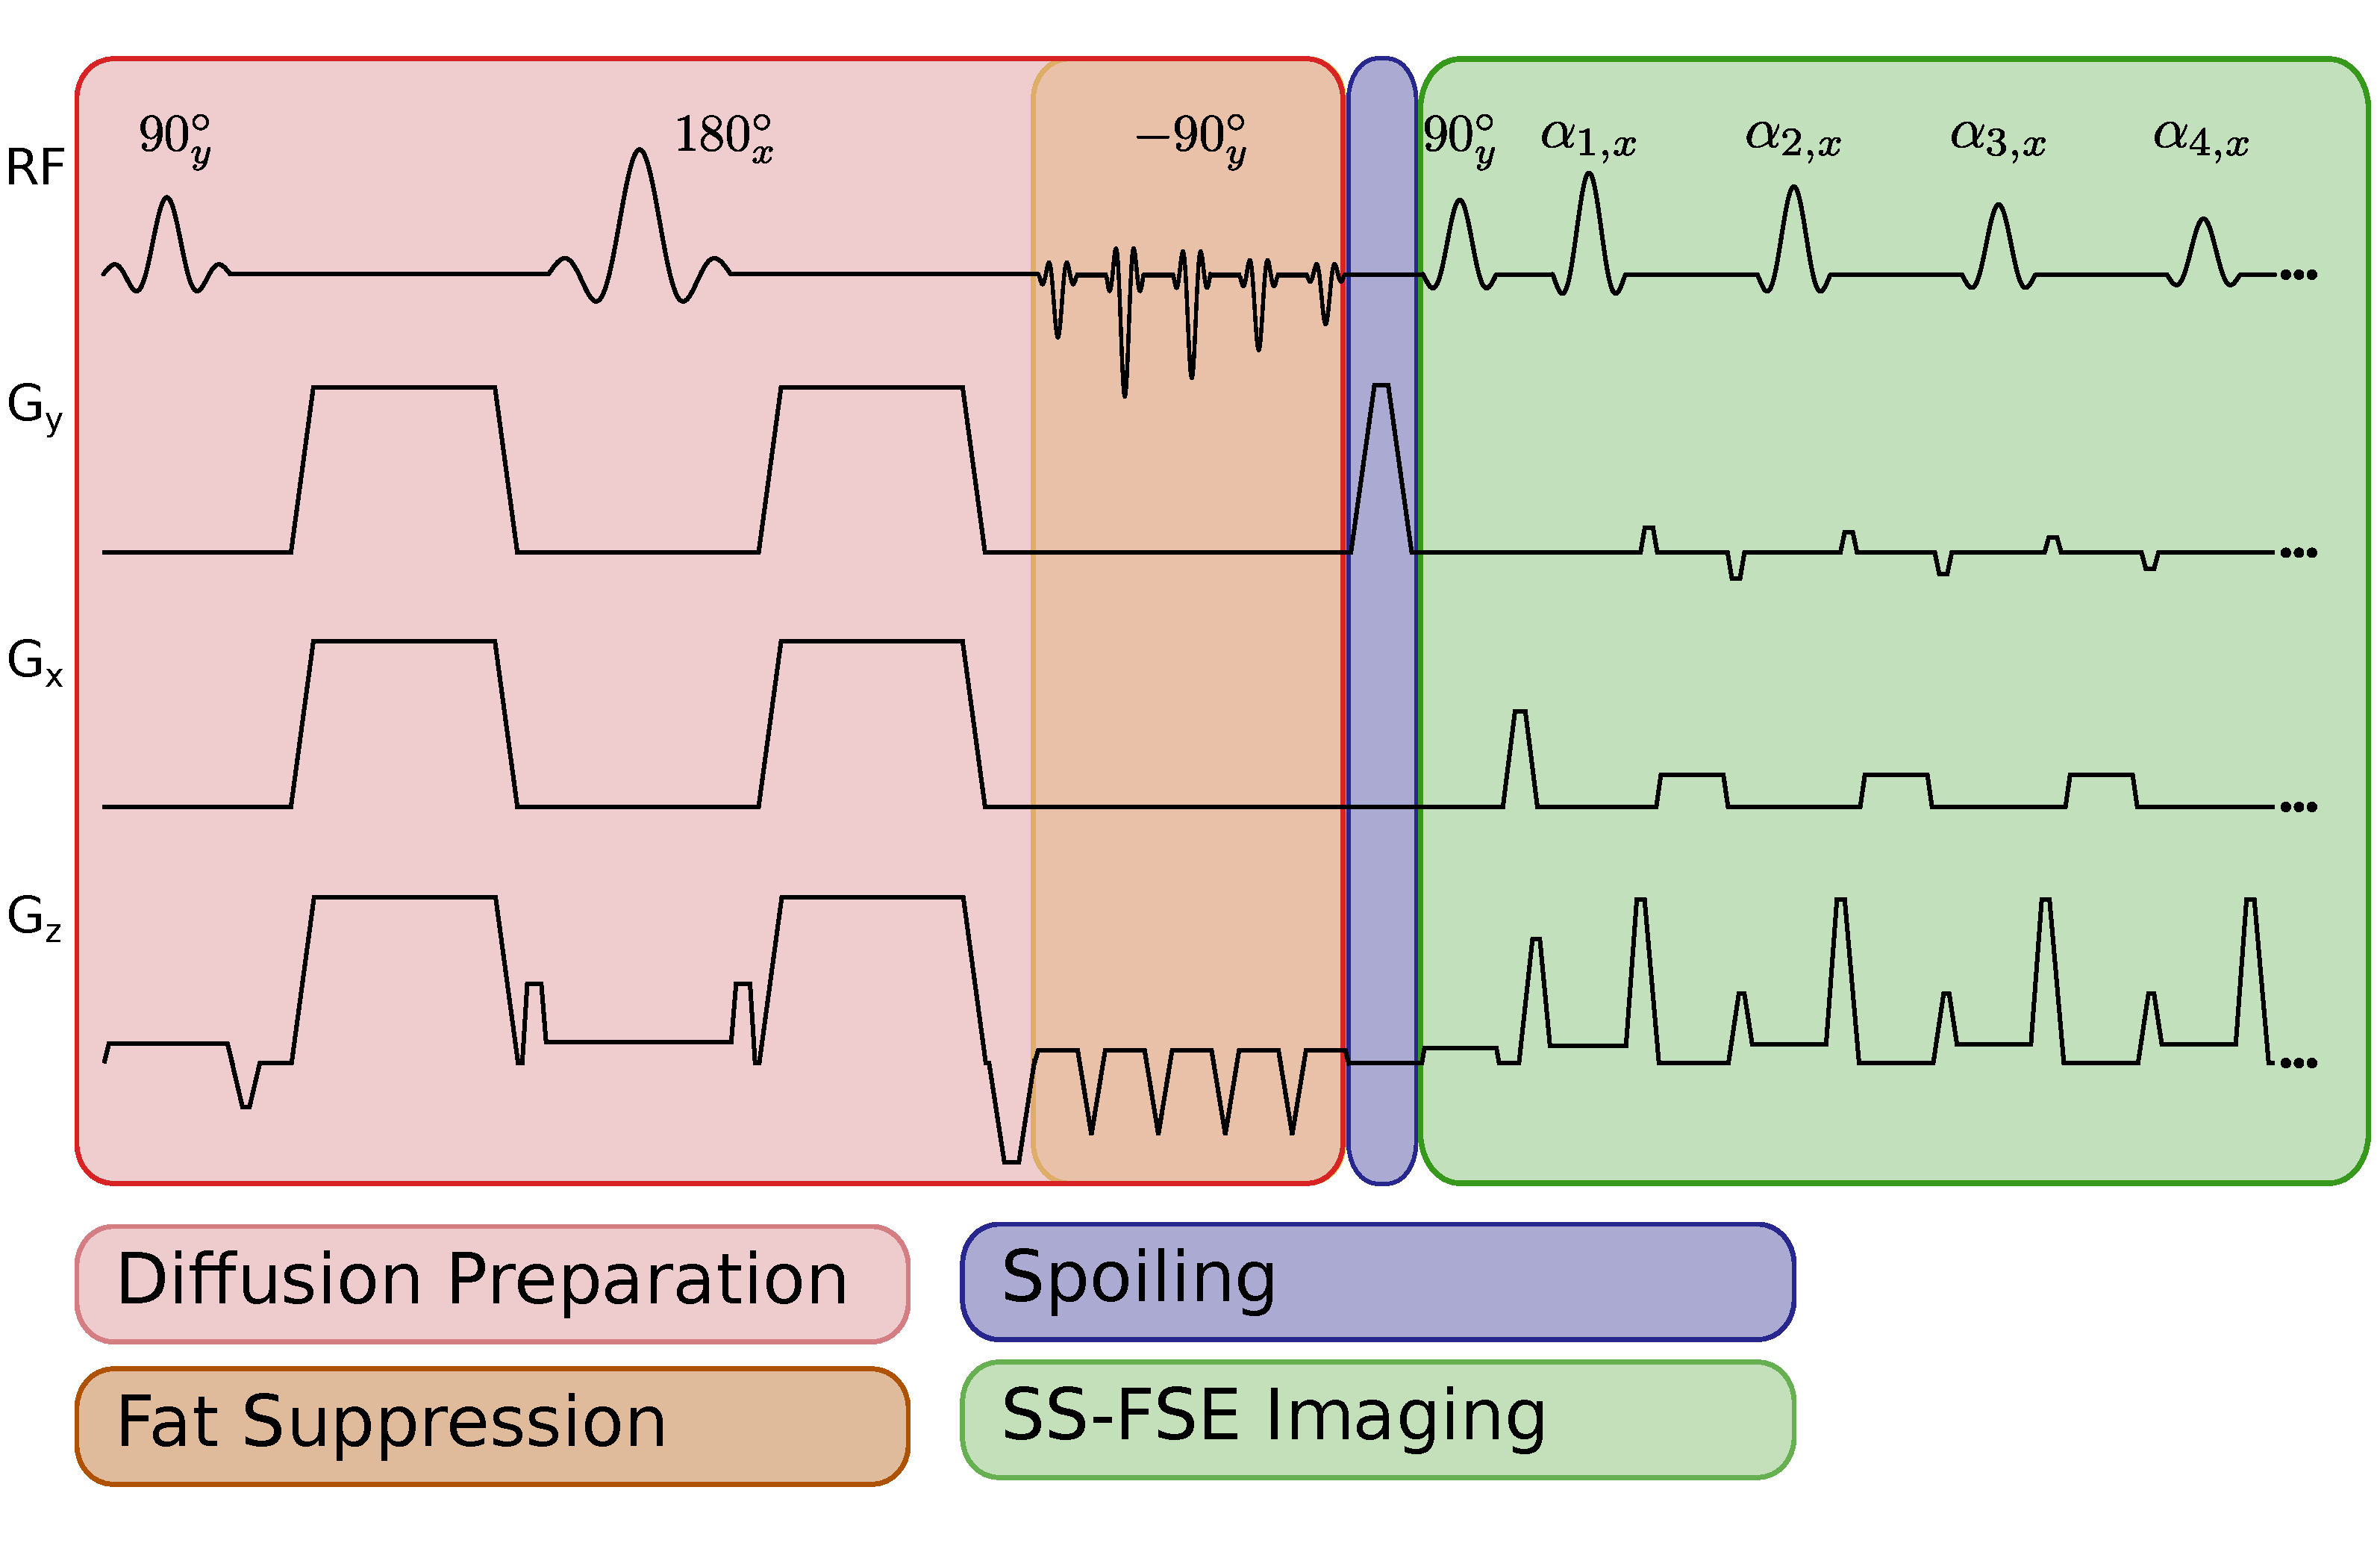
\includegraphics[width=7in]{images/gibbons_sequence.pdf}
  \caption[A very wide figure using the rotating package.]{This is an example of a wide figure that would be appropriate (maybe) for a landscape page using the rotating package.  This figure came is an MRI RF and magnetic gradient pulse sequence which is capable of generating distortion-free images with diffusion contrast.}  
  \label{fig:wideFigRotating}
\end{sidewaysfigure}

\section{Sections}
\label{sec:sections}

There are multiple levels of sections (or Headings, if you are used to MS Word).  The numbering can be toggled on and off, but keep them on for all levels for ease of searching through the document.  The highest level is a \verb+chapter+.  This current level is an example of a \verb+section+.  

\subsection{Subsections}
\label{sec:subsections}

This is an example of a \verb+subsection+.

\subsubsection{Subsubsections}
\label{sec:subsubsections}

This is an example of a \verb+subsubsection+.  This is the lowest level that \LaTeX\ supports, but if you need more granular sectioning, you might want to rethink your formatting choices.  Note that the \verb+subsubsection+ is not numbered.  



%%% Local Variables:
%%% mode: latex
%%% TeX-master: "../thesis_template_test"
%%% End:

\chapter{Another Chapter}
\label{cha:another-chapter}

Some text for another chapter...

%%% Local Variables:
%%% mode: latex
%%% TeX-master: "../thesis_template_test"
%%% End:



\appendix
\chapter{Appendix}
\label{cha:appendix}



\section{Some Long Proof}
\label{sec:some-long-proof}

This is an example appendix.

%%% Local Variables:
%%% mode: latex
%%% TeX-master: "../thesis_template_test"
%%% End:


\bibliography{mybib}
\bibliographystyle{IEEEtran}
\end{document}

%%% Local Variables:
%%% mode: latex
%%% TeX-master: t
%%% End:
